\documentclass{article}
\RequirePackage{etex} 
% Language setting
% Replace `english' with e.g. `spanish' to change the document language
\usepackage[english]{babel}
\usepackage[ruled]{algorithm2e}
\usepackage{amsthm}
\usepackage{appendix}

\usepackage[T1]{fontenc}
\usepackage{lmodern}
\usepackage{dashbox}
\usepackage[
    n,
    operators,
    advantage,
    sets,
    adversary,
    landau,
    probability,
    notions,    
    logic,
    ff,
    mm,
    primitives,
    events,
    complexity,
    asymptotics,
    keys]{cryptocode}
\usepackage{lipsum}
\usepackage{dashbox}
\usepackage{algpseudocode}
% Set page size and margins
% Replace `letterpaper' with `a4paper' for UK/EU standard size
\usepackage[letterpaper,top=2cm,bottom=2cm,left=3cm,right=3cm,marginparwidth=1.75cm]{geometry}
\usepackage{geometry}
\geometry{a4paper,scale=0.8}
\usepackage{float}
\floatstyle{plaintop}
\restylefloat{table}

% Useful packages
\usepackage{amsmath}
\usepackage{graphicx}
\usepackage[colorlinks=true, allcolors=blue]{hyperref}
\usepackage{multicol, lineno}

\newtheorem{myDef}{Definition}
\SetKwComment{Comment}{/* }{ */}

\title{Eigen ZKZRU: A Privacy-specific ZK Rollup}
\author{Eigen Labs}

\begin{document}
\maketitle


\begin{abstract}
Decentralized Privacy and security are always the most important part of Web3.0. ZCash and Monero have taken great effort to achieve privacy-enabling technology by building their private payment infrastructure and ecosystem. However, it's not easy to achieve programmable privacy on Smart Contract regarding general assets, such as ERC1155.

In this paper, we present Eigen ZKZRU, a privacy-specific ZKRollup solution on ZKRollup on Ethereum ecosystem to achieve low gas-fee, better composability and high privacy enhancement. Eigen ZKZRU proposes an Abstract Balance Leaf Model, using Twisted ElGamal encryption \cite{chen2020pgc} and Bulletproof \cite{bunz2018bulletproofs} on DDH assumption to build the confidential transaction, and constructs the validity proof of batch transaction on account Merkle tree by algebraic composite NIZK, which is built on a Two-tier architecture, the base layer is a ZKRollup, which is built on R1CS constraints system and transpiled to PLONKish Arithmetization \cite{gabizon2019plonk}, which is naturally friendly to utilize Twisted ElGamal encryption with custom gate, and hardware acceleration. The application layer is Pairing-free and easy-to-audit confidential transaction layer. 

% As a callback to our \href{https://www.eigen.cash/#/}{whitepaper}, this work gives more detail about the on-chain data privacy preservation. 

\end{abstract}

\section{Motivation}

Privacy invasion incidents become more and more frequent in Web3.0 world. Observe that the privacy of Web3.0 participants can be categorized into 3 aspects: PII\footnote{PII: Personally Identifiable Information, \href{https://en.wikipedia.org/wiki/Personal_data}{see Personal data.}}-Account Linkage, Transaction's Privacy, and Smart Contract Logic's Privacy.

Eigen Network proposes Eigen ZKZRU, a brand-new approach to implement confidential transaction on EVM-compatible blockchain. Eigen ZKZRU comes up with ABL, Abstract Balance Leaf of account tree, and applies different cryptography primitives to ABL, such as ZK Membership proof, Homomorphic arithmetics, private set interaction, and private comparator etc, thus expose the high-level private user interface to wallet. 

\subsection{Background: Privacy Issues in Web3.0}

\subsubsection{Disclosure of PII-Account linkage}

The blockchain technology provides an excellent for people to perform anonymous transaction without exposing their ID on internet, but this capability has been broken as the on-chain data analytic like Nansan and Pack Shield, more and more people are able to exploit the relationship between PII and account. Monaco's paper \cite{monaco2015identifying} 
proposed an new approach Random time-interval(RTI) model to identify and verify Bitcoin users based on the observation of Bitcoin transactions over time.  Bonifazi et.al's paper \cite{bonifazi2022defining} adopts the social network-based model to represent Ethereum and construct each user's spectrum then classify them into difference clusters on their spectra.  All those works taking efforts to link individual with their blockchain addresses deprive a user of anonymity. Furthermore, cracking the public transaction graph is big business: companies like Chainalysis and Nansen run sophisticated forensic analysis to associate various wallets, monitor activity, and make probabilistic assumptions about who owns what.

Lots of such privacy invasion incidents occurs. In this March, the Juno Network's proposal \href{https://www.mintscan.io/juno/proposals/4}{4} was submitted to voted away an whale wallet's funds to the Juno community pool and executed in proposal \href{https://www.mintscan.io/juno/proposals/16}{16}.  

\subsubsection{Vulnerable privacy and confidentiality of Smart Contract}

From the \href{etherscan.io}{Etherscan}, Not only can we see all account transactions, we can see all the amounts, assets, and counterparties. That’s in fact the power of public blockchains! Due to their public nature they are eminently auditable and verifiable. But this also leads lots heavy fairness issue in DeFi world. 

First notorious issue is \href{https://ethereum.org/en/developers/docs/mev/}{Miner Extractable Value(MEV)}. Miner extractable value (MEV) is a measure of the profit a miner (or validator, sequencer, etc.) can make through their ability to arbitrarily include, exclude, or re-order transactions within the blocks they produce.  Through MEV, Miner can make profit from exploiting the transaction in the txpool, and inserting specific transaction before or after user's transaction.

Apart from MEV, Slippage on Uniswap and other popular DEXes is a pain. Slippage is the price difference between when users submit a transaction and when the transaction is confirmed on the blockchain.  Slippage can be caused by High  trading volume or low liquidity apparently, but the one of the root causes is that miner choosing the high gas-fee transactions to confirming, and the arbitrators can leverage this and make an impact on others by increasing their gas-fee.

The decentralized Smart Contract is the core feature of Ethereum, however, the lack of confidentiality is a major hindrance towards the broad adoption of it, since financial transactions (e.g., insurance contracts or stock trading) are considered by many individuals and organizations as being highly secret. 

\subsubsection{Dilemma of utility versus privacy protection}

Tornado Cash is leading TVL on anonymous payment of Ethereum ecosystem, as a Layer 1 Dapp, supporting ERC20 only currently, and charging about 50Gwei + 100Gwei + 0.05\%~0.2\% * 0.05ETH for even a 0.05ETH transaction from source\footnote{Fee - how much does it cost to use? https://torn.community/t/fee-how-much-does-it-cost-to-use/68/3}.

Some well-known public blockchain protocols like Zerocash and Monero provide confidential transaction infrastructure but forgos programmability and unclear a primori how to enable programmability without exposing transaction and data in cleartext to miners.

Another utility issue is Nullifier is not account-friendly. The Nullifier is a public input that is sent on-chain to be checked with the smart contract and the Merkle tree data. It avoids double-spending for instance.
Because the Nullifier is irrelevant to the addresses of sender or receiver. So the receiver can do withdraw with the valid Nullifier, and cutting off the relationship between sender and the receiver.

However, this is not easy to manage such Nullifier, which is secret key for each anonymous payment transaction. 

\subsection{Vision}

Eigen Network aims to facilitate a drop-in privacy preservation protocol for every Web3 participant in EVM-compatible ecosystem.

Eigen Network focuses on building a new privacy-specific ZKRollup protocol to achieve address anonymity, smart contract data and logic confidentiality and offers users capabilities of low gas-fee confidential transaction, full Smart Contract privacy preservation and better composability of supporting most used asset like ERC20,ERC721 and ERC1166, in EVM-compatible ecosystem.

\subsection{Related Works}

There are some concurrent work to implement address anonymity, transaction and smart contract privacy preservation. 

Hawk\cite{kosba2016hawk} splits a smart contract into a public contract, which runs on-chain, and a private contract executed off-chain. Hawk requires the figure of a manager to execute the private contract. The manager must be trusted by the participants, as it can see the transactions that take place in a private contract. The manager cannot affect the outcome of the contract, it just could prevent the contract execution, or cause the abortion of the contract, and in both cases, it would be castigated.

Zether\cite{bunz2020zether} is a private transaction scheme built on top of Ethereum. It can be extended to support a limited class of smart contracts with I/O privacy—namely those that can be represented solely via homomorphic addition. This allows us to perform simple sealed-bid auctions (assuming bidders buy all units on offer) and private voting (assuming the votes are binary). Unfortunately, only transactions hiding the users' balances and the transfer amount can currently be implemented on Ethereum due to gas constraints. Unlike previous two constructions, Zether uses a "transparent" ZKP (i.e. a ZKP with no trusted setup) $\Sigma\mbox{-}Bullets$.

% Zkay\cite{baumann2020zkay} also extends Ethereum's design to support smart contracts with I/O privacy. They rely on the power of ZKPs for private computation, thus offloading the bulk of work to the user to perform offline. However, this design choice also allows them to support a larger class of functions than in Zether.

% Zexe\cite{bowe2020zexe} instead attempts to extend Zcash's design to support arbitrary coin scripts. Unlike the previous two, Zexe can also support function privacy.

The AZTEC Protocol \cite{williamson2018aztec} proposed an Join-split transactions model, and each splits is described as notes, which is UTXO-like and attached with a viewing key and spending key. and the notes can be spent in encrypted state based homomorphic arithmetic and range proof. 

Eigen Labs proposes Abstract Balance Leaf(ABL) on Account Balance Merkle Tree, and applies standard ERC20 and ERC721 operations on it based on high-level cryptography primitives, such homomorphic arithmetic and accumulator etc.

To sum up, Table \ref{tab:compare} presents the detail on privacy type, approach, expressivity and which blockchain protocol to extend.  

\begin{table}
\resizebox{\textwidth}{!} {
\begin{tabular}{c|c|c|c|c}
Scheme & Privacy type & Approach & Expressivity & Extension as \\\hline
Hawk & I/O & Offchain MPC/TEE & Arbitrary functions & Ethereum L1 \\
Zether & I/O & Elgamal and $\Sigma$-Bullet & Additive functions & Ethereum L1\\
AZTEC & I/O, function & Pairing based homomorphic Commitment & Additive functions & Ethereum L2\\
Eigen ZKZRU & I/O, function & Pair-free Homomorphic PKE and Bulletproof & Arbitrary functions & Ethereum L2
\end{tabular}
}
\caption{\label{tab:compare}A comparison of Privacy-preserving Smart Contract Scheme}
\end{table}

For privacy type, I/O is corresponding short for Encrypted Input/Output. If end user encrypts the input, and send it to the miner to run the contract, it would be Encrypted Input. Otherwise, the end user need run the contract locally with clear input and encrypts the output, then sends the encrypted output to miners.

There are different approaches to obtain privacy enhancement, The classic methods include Homomorphic arithmetic or some commitment scheme, TEE, MPC and NIZK. Homomorphic arithmetic is deeply limited to to performance in computation, especially fully homomophgic encryption, so the practical approaches would be commitment scheme, like additive or multiplicative to perform special operations like \textbf{Split} and \textbf{Join} in AZTEC Protocol. The MPC needs large of communication complexity and this raises complex interoperability between on-chain and off-chain. The TEE uses special hardware to achieve computing efficiency and code integrity. NIZKs, Non-interactive zero-knowledge proofs, enable a party, known as the prover, to convince another party, known as the verifier, about knowledge of the witness for an NP statement without revealing any information about the witness (besides what is already implied by the statement being true). 

Expressivity is the scope of the scheme being able to protect.

A deep comparison with AZTEC from implementation perspective on acceleration and architecture in Table \ref{tab:widgets2}. Eigen ZKZRU leverages decentralized proof-Of-Proving mechanism to accelerate the proving computation, and it's naturally for us to utilize hardware acceleration, too, such as GPU and ASIC for NTT computation in polynomial commitment and multi-scalar multiplications on elliptic curves. The second difference is we adopt Stealth Address to implements the address anonymity.

\begin{table}
\centering
\begin{tabular}{c|c|c}
Capabilities $\backslash$ Projects & Eigen ZKZRU & AZTEC ZK-ZKRollup \\\hline
EVM Compatibility & Partial/Language Level & Partial/Language Level \\

Prover Decentralization & \color{red} Decentralized Eigen Relayer & Wasm in Browser \\
Circuit DSL & Circom & Noir \\
Prove System & Plonk & Plonk \\
Recursive Proof & Yes & Yes \\
GPU acceleration enable & \color{red} Yes & No \\
Anonymous Address & \color{red} Stealth Address & Nullifier \\

\end{tabular}
\caption{\label{tab:widgets2} A comparison between Eigen Network and AZTEC Network}
\end{table}


\section{Eigen ZKZRU Design Rationale}

Eigen ZKZRU aims to facilitate a drop-in privacy preservation application for every Web3 participant in EVM-compatible ecosystem, provides user the capacities as below.

\noindent\textbf{Low Gas-fee}. Free deposit, Batch transfer by ZK-Rollup, Low gas-fee withdrawal.

\noindent\textbf{Composability}. Not only ERC20,  both ERC721 and Swap are supported.

\noindent\textbf{Privacy Enhancement}. Confidential transaction and address anonymity based on ZK-ZKRollup  

\noindent\textbf{Easy-to-use}. Self-custodial Secret(Private Key/Secret words) Management and Multisig Wallet based Account Abstract.


\subsection{Overview of Eigen ZKZRU}

Eigen ZKZRU is a Two-Tier architecture, the base layer is ZKRollup layer, which empowers applications with zero-knowledge proofs. The upper layer is the confidential transaction layer, which provides high-level interface of confidential asset, which is pegged to the token in Layer 1. The Two-Tier architecture is necessary due to two factors as below.

\noindent\textbf{Privacy-oriented protocol}. Eigen ZKZRU is to provide a privacy "Lego" for end-users to protect their asset's confidentiality and security before the asset flowing into other liquidity pool or protocols in DeFi world. Differ from the zkEVM solution, such as ZKSync, we can deploy our confidential transaction layer on other ZKRollup L2s. Hence we design the transaction layer on pair free cryptography scheme to try best to save the gas and lower the implementation complexity, and for privacy concern, we need to generate the Zero-knowledge transaction in user-side, like by browser.

\noindent\textbf{Acceleration of ZK Proving}. Proving a computation requires first translating it from a classical program to a ZK-friendly format, then use proof system, such as Groth16, Plonk, STARK, to generate the validity proof. No matter which proof system used, the bottleneck always ends up being either:

% https://www.paradigm.xyz/2022/04/zk-hardware
\begin{itemize}
    \item Multiplications over large vectors of number on Group or Fields, especially variable-base and fixed-base multi-scalar multiplications (MSMs);
    \item Fast Fourier Transforms (FFTs) and Inverse FFTs (although there are techniques for FFT-less proof systems).
\end{itemize}

In systems where both FFTs and MSMs exist, about 70\% of the time generating a proof is spent on MSMs, and the rest is dominated by FFTs. There are some methods to improve the performance, but hardware acceleration does really matter.  For the ZKRollup layer, we design a the proof-of-proving model for miner to participant in the computation, and the miner would provide powerful and optimized computation.


\subsubsection{Base Layer: ZK Rollup}

The ZK Rollup is a very promising approach to scale Ethereum.  The ZK Rollup consists of Rollup contract and A off-chain proving nodes. The Rollup contract maintains a transaction Merkle tree root list and a account Merkle tree. The proving nodes act as:
\begin{itemize}
    \item a RPC server for user to interact with ZK Rollup
    \item a sequencer to sort the transaction and generates the transaction Merkle tree root, submit the root into L1 Rollup contract
    \item a prover to generate the Rollup block validity proof, and update the global account Merkle tree.
\end{itemize}

% The node  data validity, collecting transactions, and bundling up the transactions into a batch, and submits the Merkle proof into L1 contract. which means putting them into a consistent, global incremental order with no gaps. 

The prover generate the validity proof by the \href{https://github.com/ieigen/EigenZKit}{EigenZKit}. EigenZkit is our ZKRollup \textit{compiler}, which make it easy for the developer to write constraints by Circom, transpile the circuits to PLONKish Arithmetization \cite{gabizon2019plonk}, optimize the proving with the Lookup table and aggregation proof, and finally generate the proof and solidity verifier on Plonk argument. 

The rollup contract maintains a state root: the Merkle root of the state of the Rollup (meaning, the account balances, contract code, etc, that are "inside" the rollup). And check the validity of the new proof with public input transaction Merkle tree root and new account Merkle tree root.

The basic data representation of rollup blockchain's world state see Figure \ref{fig:zkzru}. The depth could be scaled to 28 or larger, which means our ledger merkle depth can reach up to $2^{28}$ accounts.

\begin{figure}
    \centering
    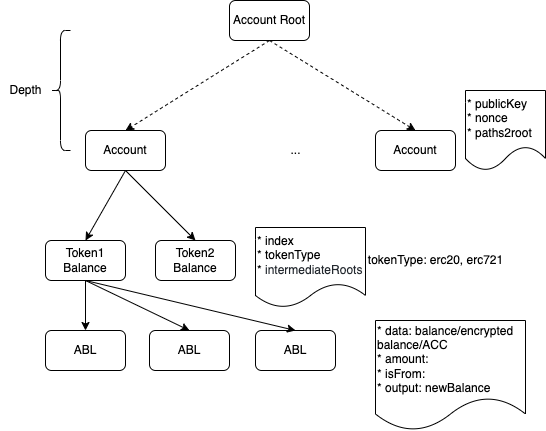
\includegraphics[width=0.6\textwidth]{zkzru.drawio.png}
    \caption{\label{fig:zkzru}ZKRollup Account Tree}
\end{figure}

\subsubsection{Confidential Transaction Layer: Abstract Balance Leaf Model}
To achieve the goal of transaction confidentiality, we proposes an Abstract Balance Leaf Model. Similar to the "note" in AZTEC, The ABL is also an encrypted representation of abstract value, which maps into high-level digital asset deposited into Eigen ZKZRU. The ABL is an output of the Eigen ZKZRU encryption value from formula \ref{f1}. 
% The core difference from previous work is that Eigen ZKZRU use Merkle Tree to sepreate the assert owner and data representation, and extends the token type and supports general standards like ERC20, ERC721 and ERC1155 etc. Depends on ABL, we can also construct Zexe\cite{bowe2020zexe} like scheme in the future to support general ZKRollup. 

The specific protocol of Confidential Transaction Layer will be presented in section \ref{section:fundanmental}, \ref{section:abl} and \ref{section:pay-abl}.

\subsection{Fundamental} \label{section:fundanmental}

Pedersen commitment \cite{pedersen1991non} uses random public generators $\GG$ and $H$ of a suitable large group where the DDH\ref{d:ddh} is hard, for making a blinded, non-interactive commitment to a value. Eigen ZKZRU use Elliptic Curve Pedersen Commitment to hide the secret. Worth to note that we use native Pedersen commitment scheme to describe our algorithm in this paper for easy understanding, and implements by Elliptic Curve Pedersen Commitment.

\begin{myDef}
\label{d:dla}
\textbf{Discrate logarithm assumption.} Let $\GG$ be a group of prime order q, a generator $g \in \GG$ and an arbitrary element $y \in \GG$, it's infeasible to find $x \in ZZ_p$, such that $y = g^x$.
\end{myDef}

\begin{myDef}
\label{d:ecpc}
\textbf{Elliptic Curve Pedersen Commitment\cite{francca2015homomorphic}}. An efficient implementation of the Pedersen Commitment will use secure Elliptic Curve Cryptography (ECC), which is based on the algebraic structure of elliptic curves over finite (prime) fields. Let $F_p$ be the
group of elliptic curve points, where p is a large prime. Also, let $\GG$ be the base point of EC, and ${H}$ be another EC point, and the discrete logarithm of H no one has to know (H = qG). Attackers who know q can produce valid proofs without knowledge of x. To commit to a value $x \in \ZZ_p$, we pick a random integer $r \in \ZZ_p$ and calculate the commitment as:
$$
Com(x, r) = xG + rH
$$
To open the commitment we simply reveal the values x and r. EC Pedersen is also additive homomorphic, so it has the following properties:
\begin{equation}
\begin{split}
Com(x + y, rx + ry) &= Com(x, rx) + Com(y, ry) \\
Com(k \cdot x, k \cdot r) &= k \cdot Com(x, r)
\end{split}
\end{equation}

EC Pedersen Commitment could be used for hide several values in following way:

\begin{equation}
    C(r, \overline{a}) = rH + a_1G_1 + a_2G_2 + ... + a_nG_n
\end{equation}
where each $G_n$ has to be formed using NUMS\cite{black2014elliptic} approach. 

\end{myDef}


\begin{myDef}
\label{d:ddh}

\textbf{Decisional Diffie-Hellman assumption}. Given some group \GG, and element element $g$, and the elements $g^a$, $g^b$ and $g^{c}$, determine whether $g^{ab} = g^c$, The DDH assumption holds if for any PPT adversary \adv, we have: 
\begin{equation}
    Pr[\adv(g, g^a, g^b, g^{ab}) = 1] - Pr[\adv(g, g^a, g^b, g^c) = 1] \leq \negl[\lambda]
\end{equation}

\end{myDef}

\begin{myDef}
\label{d:zkp}
\textbf{A Non-interactive Zero-knowledge(NIZK) proofs}. A zero-knowledge proof of a statement does not reveal any information beyond the validity of the statement. A NIZK proof system for input $x$ in language L, with witness $w$, is a set of efficient PPT algorithms (K, P, V) such that:
\begin{enumerate}
    \item Setup: generates the common reference string on security parameters $\lambda$, $pp \gets K(1^\lambda)$.
    \item Prover: $\pi \gets P(pp, x, w)$ produces the proof.
    \item Verifier: $V (pp, x, \pi)$ outputs {0, 1} to accept/reject the proof.
\end{enumerate}
Which satisfy the completeness, soundness, and zero-knowledge properties. 

\noindent\textbf{Completeness}. $\forall x \in L, w \in R_L$, such that:
\begin{equation}
    Pr[pp \gets K(1^{\lambda}); \pi \gets P(pp, x, w): V(pp, x, \pi) = 1] = 1
\end{equation}
\noindent\textbf{Soundness}. Assume x can be decided when seeing $pp$.
\begin{equation}
    Pr[pp \gets K(1^{\lambda}); \exists (x,\pi), s.t. V(pp, x, \pi) = 1] = \negl[\lambda]
\end{equation}
\noindent\textbf{Zero-knowledge}. There exists a PPT simulator split into two stages $S_1, S_2$ such that for all PPT attackers $A$, the two distributions are computationally indistinguishable:

\begin{pchstack}[ center , boxed ]
\pseudocode [ linenumbering ]{
pp \rightarrow K \\
(x, w) \gets A(pp), s.t. (x, w)\in R_L \\
\pi \gets P(pp, x, w) \\
output (pp, x, \pi) }
\end{pchstack}

% \begin{enumerate}
% \item $pp \rightarrow K$
% \item $(x, w) \gets A(pp)$, s.t. $(x, w)\in R_L$
% \item $\pi \gets P(pp, x, w)$
% \item output $(pp, x, \pi)$
% \end{enumerate}

And the simulator output:

\begin{pchstack}[ center , boxed ]
\pseudocode [ linenumbering ]{
(pp, \tau) \rightarrow S_1(1^\lambda) \\
(x, w) \gets A(pp), s.t. (x, w)\in R_L  \\
\pi \gets S_2(pp, x, \tau) \\
output (pp, x, \pi) }
\end{pchstack}

Where $\tau$ should be thought of as local state stored by the simulator (passed between stages).
\end{myDef}


\subsection{Abstract Balance Leaf Model} \label{section:abl}

\textbf{Paring based cryptography vs ECC based cryptography}.  Pairing-based cryptography(PBC) is a function that maps a pair of points on an elliptic curve into a finite field to construct or analyze cryptographic systems. Bilinear pairings can be used to transport the discrete logarithm problem on a certain class of elliptic curves over a finite field to the discrete logarithm problem on a smaller finite field. PBC is widely used in ZKP, such as the KZG commitment, Groth16 and Plonk etc. However, pairings are notoriously expensive in implementation complexity and processing time, and this is not very friendly to confidential transaction on ZKRollup. Therefore, we try to use the ECC based scheme to implement the confidential transaction layer.

~\\
\noindent\noindent\textbf{Commitment Scheme VS Public Key Encryption}. Pure commitment-based approach suffers from several issues due to lack of decryption capability, senders are required to honestly transmit the openings of outgoing commitments (includes randomness and amount) to receivers in an out-of-band manner. This issue makes the system much more complicated, as it must be assured that the out-of-band transfer is correct and secure. Second, users must be stateful since they have to keep track of the randomness and amount of each incoming commitment. To solve this, AZTEC utilizes set membership proof commitment scheme \cite{camenisch2008efficient,arfaoui2015practical}, defining a new commitment scheme $ Com(k; a) := (\mu_k^a, \mu_k^{ka}h^a)$ on $[1; k_{\mbox{MAX}}] \times \ZZ_p^{*} \longrightarrow \GG \times \GG$, where $a$ is random in $\ZZ_p$ and $h$ is generator of group $\GG$, and hide the balance in commitment. This scheme need a universal trust setup.  On the other hand,  Zether built the confidential transaction on ElGamal Encryption\cite{elgamal1985public}, which provides addictive homomorphic, computational hiding and unconditionally binding. Zether proposed $\Sigma\mbox{-}bullets$ to bridge the interoperability between $\Sigma\mbox{-}protocol$ and Bulletproof\cite{bunz2018bulletproofs}, with no trust setup. However the brute-force enumeration is necessary to find out the clear balance m on $g^m$ in the extreme case that the receiver received an unknown balance from sender.

Another recent work \cite{chen2020pgc} proposed PGC(Pretty Good Confidentiality) scheme on twisted ElGamal scheme, admits transparent setup, and its security is based solely on the widely-used discrete logarithm assumption. 

~\\
\noindent\textbf{Twisted ElGamal encryption \cite{chen2020pgc}}. Twisted ElGamal encryption is a public key encryption scheme improved based on the simplified version of the ElGamal. Twisted ElGamal encryption retains additive homomorphism and is as efficient and secure as the standard exponential ElGamal. More importantly, it is zero-knowledge friendly. Note that the second part of twisted ElGamal ciphertext can be viewed as Pedersen commitment [9] under the same commitment key, whose DL (discrete logarithm) relation is unknown to all users. Such structure of twisted ElGamal makes it compatible with all zero-knowledge proofs whose statement is of the form Pedersen commitment. In particular, one can directly employ Bulletproofs\cite{bunz2018bulletproofs} to generate range proofs for values encrypted by twisted ElGamal in a black-box manner, and these proofs can be easily aggregated. Therefore, Twisted ElGamal enables us to easily devise zero-knowledge proofs for essential correctness of transactions and various application-dependent policies in a modular fashion. 

Moreover, twisted ElGamal is very efficient. Compared with the most efficient reported implementation of Paillier PKE, twisted ElGamal is an order of magnitude better in key and ciphertext size and decryption speed (for small message space), two orders of magnitude better in encryption speed. Consequently, we achieve an efficient and effective protection approach for account privacy by designing a twist EIGamal-based homomorphic encryption scheme.

Eigen ZKZRU extends a twisted ElGamal encryption on elliptic curve, and combines with \href{https://datatracker.ietf.org/doc/html/rfc8032}{EdDSA signrature} scheme to , and optimizes the Camenisch and Stadler \cite{camenisch1997efficient} notation for proofs of knowledge \ref{f1}. This scheme can be easily proved that it holds the unconditionally hiding and computational binding same as Pedersen Commitment by the work from \cite{bunz2020zether,chen2020pgc} on the DDH Assumption. Hence, the final proof of Zero-knowledge scheme would be as follow in formula \ref{f1}.

\begin{equation}
 PK\{(m, k, r): PK = g^k \land (X, Y) = (PK^{r}, g^r h^m)\} \land (0 \leq m < \mbox{MAX}) \label{f1}  
\end{equation}

There are four primary algorithms in twisted ElGamal, as presented below.

\textbf{\pgen($1^\lambda$)} $\lambda$ is security parameter.  Run the Gen($1^\lambda$), choose another generator element $h \sample \GG$. Output pp = (G, g, h, p) as global public parameters.

\textbf{$\kgen($pp$)$} On input $pp$, choose a secret key $sk \sample \ZZ_p$, and set the public key $pk = g^{sk}$.

\textbf{\enc(pk, m)} on input the public key pk and a message $m \in  M$: pick random $r \sample \ZZ_p$, compute $X=pk^r, Y = g^r \cdot h^m$

\textbf{\dec(sk, C=(X,Y))} , calculate $h^m = {Y}/{X^{\frac{1}{sk}}}$,  then figure out m from $h^m$ by brute-force enumeration with time complexity $\bigO{\mbox{MAX}}$, where $\mbox{MAX}=2^{31}$. The Baby-step/Giant-step algorithm \cite{Shanks1971ClassNA} with an efficient table lookup scheme would decrease it to $\bigO{\sqrt{\mbox{MAX}}}$.

The above scheme can be proved \indcpa\ secure(1-plaintext/2-recipient) base on the divisible DDH assumption from \cite{chen2020pgc}.

Furthermore, we construct the set membership proof on this scheme from the work \cite{camenisch2008efficient} and Boneh-Boyen signatures \cite{jao2009boneh}, and extend it to a pairing free scheme in Appendex \ref{appendex: bbs-no-pairing}.

~\\
\noindent\textbf{Edwards-curve Digital Signature Algorithm}. Edwards-curve Digital Signature Algorithm (EdDSA\footnote{EdDSA: https://datatracker.ietf.org/doc/html/rfc8032}) is a digital signature scheme using a variant of Schnorr signature based on twisted Edwards curves. It is designed to be faster than existing digital signature schemes without sacrificing security. The sketch of EdDSA is presented in Algorithm \ref{eddsa}.

\begin{algorithm}
 \caption{EdDSA signature generation (sketch)}
 \label{eddsa}
 \LinesNumbered
 
 \KwIn{Group parameters ($\GG, g, p$), signer’s key pair ($sk, pk = g^{sk}$), signer’s long-term secret n for session-key generation, and message M, pick cryptographic hash function H: $M \times \GG \rightarrow \ZZ_p$}
 \KwOut{Signature (R, s) of M}
 $r \gets H(n, M) \mod{p}$ \;
 $R \gets rG$ \;
 $h \gets H(R, M) \mod{p}$ \;
 $s \gets r + h \cdot sk \mod{p}$ \;
  return (R, s)
\end{algorithm}

~\\
\noindent\textbf{Zero-knowledge proofs on ABL}. In ABL model, we ensure that the encrypted transaction are correct by using ZKP that claiming correctness without revealing any additional information. Since twisted ElGamal compatible with all zero-knowledge proofs whose statement is of the form Pedersen commitment, we can directly employ Bulletproof to generate the balance's range proof. 

We define the a language $L_{transfer}$ to describe our ABL model in definition \ref{l_transfer}.

\begin{equation}\label{l_transfer}
\begin{aligned}
    L_{transfer} &= \{((pk_s, pk_r, C_s, C_r, sk_s, v, r_1, r_2)) | \\ 
        pk_s &= sk_sG \land C_s = \mbox{HPKE}.Enc(pk_s,v, r_1) \land \\
        C_r &=  \mbox{HPKE}.Enc(pk_r,v, r_2) \land v \in [0, \mbox{MAX}) \land \\
        &\mbox{HPKE}.Dec(sk_s, \hat{C}_s - C_s) \in [0, \mbox{MAX})\}
\end{aligned}
\end{equation}

The conjunction of $L_{transfer}$ is $\pi_{transfer}$, the sketch of the prove process is described as below in Figure \ref{fig:pi_transfer}.
\begin{figure}[H]
    \centering
    \caption{Caption}
    \label{fig:pi_transfer}
\dbox{%
\procedure[linenumbering]{Proof sketch: $\pi_{transfer}$}{
\textbf{Prover} \> \> \textbf{Verifier} \\
w \gets (r, v) \> \> \\
a, b \sample \ZZ_p \> \> \\
A_1 \gets pk_1^a, A_2 = pk_2^b, \> \> \\
B \gets g^ah^b \> \> \\
\> \sendmessageright*{\scriptsize A_1, A_2, B} \> \\ 
\> \> e \sample \ZZ_p \\
\> \sendmessageleft*{\textbf{\scriptsize e}} \> \\ 
z \gets a + er \>\> \\
t \gets b + ev \>\> \\
\> \sendmessageright*{\scriptsize z, t} \> \\ 
\> \>  \mbox{check if} \\
\> \>  pk_1^z = A_1X_1^e \\
\> \>  pk_2^z = A_2X_2^e \\
\> \>  g^zh^t = BY^e 
}
}
\end{figure}

\subsection{Payment Mechanism over Abstract Balance Leaf} \label{section:pay-abl}

We use Twisted ElGamal encryption \cite{chen2020pgc} and Bulletproof \cite{bunz2018bulletproofs} on DDH assumption to build the confidential transaction, and constructs the validity proof of batch transaction on account Merkle tree by algebraic composite NIZK. Without lose the generality, we also implement set membership proof on our scheme naturally, to support general asset private payment, such as ERC721, and ERC1155, Eigen ZKZRU extends the ABL, and proposal Zero-knowledge computation on ABL to support non-fungible transaction, order-based token exchange etc. For instance, the state in ERC20 token would be describe as below after after transaction $t$ in Table \ref{tab:transfer}. 

\begin{table}
\centering
\begin{tabular}{l|l|l}
public key & balance(ABL) & constraints \\
\hline
... & ... & ...  \\
\hline
$y_{Alice}$  & Comm($b_{Alice} - b_t$, $y_{Alice}$) & $b_{Alice} - b_t \ge 0$ \\
\hline
$y_{Bob}$  & Comm($b_{Bob} + b_t$, $y_{Bob}$) & $b_{Bob} + b_t \ge b_{Bob} $  \\
\hline
$y_{Cathe}$  & Comm($b_{Cathe}, y_{Cathe}$) & ...   \\
\end{tabular}
\caption{\label{tab:transfer}Simple Confidential Transaction Example}
\end{table}

To stimulate above computation regarding of the constraints, we use homomorphic PKE to encode the balance and transfer amount, use NIZK to enforce senders to build confidential transactions honestly and make validity publicly verifiable, and use digital signature to authenticate transactions. Let $HPKE = (Setup, KeyGen, Sign, Verify, Enc, Dec)$ be homomorphic PKE integrated with EdDSA signature scheme on message space $\ZZ_p$, the $HPKE$ uses same key for encryption and signing, which proposed a general construction from \cite{paterson2011joint}. And let $NIZK = (Setup, CRSGen, Prove, Verify)$ be a NIZK proof system. The privacy-preserving payment mechanism consists of a trusted setup, user algorithm and a smart contract.

\textbf{Setup}. The setup algorithm calls $Setup_{nizk}$ and $Setup_{nizk}$ as subroutines, which are the setup algorithms for the proof system and the signature scheme, respectively. The former setup could depend on the relations for which proofs are constructed. If these subroutines are trustless, then the whole setup is trustless, meaning that its correctness can be verified publicly. we use Plonk argument and EDDSA, the Plonk argument needs an trust setup and EDDSA is trustless.

Setup algorithm is formally described in Algorithm \ref{alg:setup}. Apart from setting up the proof system and signature scheme, it initializes account tree accountTree, minc contract, token registry contract, a last roll over epoch updateNumber to keep track of the last epochs accounts were updated, The setup also specifies an epoch length E and a \mbox{MAX}imum amount value \mbox{MAX}.

\begin{algorithm}
 \caption{Payment Mechanism on ABL: Setup}
    \label{alg:setup}
    \LinesNumbered
    
    \KwIn{Security parameter $\lambda$}
    $pp_{hpke} \gets \mbox{HPKE.Setup}(1^\lambda)$ \;
    $pp_{nizk} \gets \mbox{NIZK.Setup}(1^\lambda)$ \;
    $crs \gets \mbox{NIZK.CRSGen}(pp_{nizk})$ \;
    $pp = (pp_{hpke}, pp_{nizk}, crs)$ \;
    Initialize {
        \begin{itemize}
            \item[$-$] account Merkle tree contract: accountTree
            \item[$-$] MiMC contract: mimc
            \item[$-$] token registry address: tr
            \item[$-$] updates and updateNumber for keeping track of the rollup blockchain
            \item[$-$] transaction Merkle tree root array: txRoots
        \end{itemize}
    }
    Deploy Rollup contract with parameters $pp$, accountTree, txRoots, minc, tr, \mbox{MAX}, BAL\_DEPTH, TX\_DEPTH
    
\end{algorithm}

\textbf{User algorithm}. A user can run one of the following algorithms to interact with the smart contract. The output of these algorithms are raw transactions. We leave it implicit that they will be signed (using the public key of the Ethereum account from which they are sent) and destined to the Eigen ZKZRU smart contract. All the algorithms get the security parameter as input but we show it explicitly only for the first one. The algorithm is presented in 
Algorithm \ref{alg:payment_mechanism}.

\begin{algorithm}
 \DontPrintSemicolon
 \LinesNumbered
 \caption{Payment Mechanism on ABL: User algorithm} \label{alg:payment_mechanism}
    \KwIn{$pp_{nizk}, pp_{hpke}, (\GG, p, g, h)$}
    
    % \begin{multicols}{2}

    \SetKwFunction{FCreateAccount}{CreateAccount}
    \SetKwFunction{FCreateTX}{CreateTX}
    \SetKwFunction{FBalanceOf}{BalanceOf}
    \SetKwFunction{FVerifyTX}{VerifyTX}
    
    \SetKwProg{Fn}{Function}{:}{}
    \Fn{\FCreateAccount{$\hat{v}, sn$}}{
        $sn \in \{0, 1\}^n$ \;
        $(sk, pk) \gets \mbox{HPKE.KeyGen}(pp_{HPKE})$ \; 
        $\hat{C} \gets \mbox{HPKE.Enc}(pk, \hat{v}, r)$ \;
        \KwRet{ $sn, (sk, pk), \hat{C}$}
    }
    
    \SetKwProg{Fn}{Function}{:}{}
    \Fn{\FCreateTX{$sk_s, pk_s, v, pk_r$}}{
        $r_1, r_2 \sample \ZZ_p$ \;
        $C_s \gets \mbox{HPKE.Enc}(pk_s, v; r_1)$ \;
        $C_r \gets \mbox{HPKE.Enc}(pk_r, v; r_2)$ \;
        $memo \gets (pk_s, pk_r, C_s, C_r) \in L_{transfer}$ \;
        $w \gets (sk_s, v, r_1, r_2)$ \;
        $\pi_{transfer} \gets \mbox{NIZK}.Prove(memo, w)$ \;
        $\sigma \gets \mbox{HPKE}.Sign(sk_s, sn, memo, \pi_{transfer})$ \;
        \KwRet { sn, memo, $\pi_{transfer}, \sigma$ }
    }

    \SetKwProg{Fn}{Function}{:}{}
    \Fn{\FBalanceOf{$sk, \hat{C}$}}{
        $\hat{v} \gets \mbox{HPKE.Dec}(sk, \hat{C})$ \;
        \KwRet {$\hat{v}$}
    }
    
    \SetKwProg{Fn}{Function}{:}{}
    \Fn{\FVerifyTX{sn, memo, $\pi_{transfer}, \sigma$}}{
        $output_1 \gets sn \ge sn^* $ \;
        $output_2 \gets \mbox{HPKE.Verify}(pk_s, (sn, memo, \pi_{transfer}, \sigma))$ \;
        $output_3 \gets \mbox{NIZK.Verify}(crs. memo, \pi_{transfer})$ \;
        \KwRet{$output_1 \land output_2 \land output_3$}
    }
    % \end{multicols}
\end{algorithm}


\textbf{Smart Contract}. The Smart Contract describe how users interact with Eigen ZKZRU. \textit{Deposit} deposits the token on Rollup contract, and mint on L2, \textit{Withdraw} does the exact opposite by burning the token on L2 and returns the token left back to L1. \textit{Transfer} does the updates the cipher balance of both sender and receiver, and creates the proof $\pi_{transfer}$ for the state transition on L2.  \textit{BalanceOf} returns the clear balance of the account, and \textit{UpdateAccountTree} generates the proof for each transaction batch, and updates the Rollup chain, which is maintained in Rollup contract.

In our scheme, users need generate a new key pair for each transaction, the private key acts as the blinding factor for the new commitment of the new transaction, and update previous blinding factors locally.


\begin{algorithm}
 \DontPrintSemicolon
 \LinesNumbered
 \caption{Payment Mechanism on ABL: Smart Contract}
  \begin{multicols}{2}
  
  \SetKwFunction{FDeposit}{Deposit}
  \SetKwFunction{FWithdraw}{Withdraw}
  \SetKwFunction{FTransfer}{Transfer}
  \SetKwFunction{FBalanceOf}{BalanceOf}
  \SetKwFunction{FUpdateAccTree}{UpdateAccTree}
  \SetKwFunction{FUpdateTxTree}{UpdateTxTree}

  \SetKwProg{Fn}{Function}{:}{}
  \Fn{\FDeposit{$b, \hat{C}, R, type, sn$}} {
    \tcp{amount $b$}
    \tcp{ encrypted amount $\hat{C}$}
    \tcp{ blinding factor $R = h^r$}   % TODO leak
    \tcp{ token type $type$}
    \tcp{ serial number $sn$ }

    \eIf {$type = 0$} {
        require msg.value = 0 $\land$ b = 0 \;
    } {
    \eIf{$type = 1$} {
        require b $\ge$ 0 $\land$ msg.value $\ge$ b \;
        transfer(ETH, msg.sender, address(this), $b$)
    } {
        \tcc{transfer ERC20 token}
        transfer(tokenAddress, msg.sender, address(this), $b$)
    }
    }
    
    $(X, Y) = \hat{C}$ \; 
    $Y \overset{?}{=} g^b \cdot R$ \;
    amountComm = $\hat{C}$ \;
    depositHash = mimc.hash([y, amountComm, $type$]) \;
    accountTree.insertLeaf(depositHash) \;
    st = accountTree.getRootFromProof()
    \KwRet{st}
  }
  
  \SetKwProg{Fn}{Function}{:}{}
  \Fn{\FWithdraw{$pi_{withdraw}, txinfo, pk_r, b$}} {
    \tcp{withdrawProof $pi_{withdraw}$}
    \tcp{transaction info $txInfo$}
    \tcp{recipient $pk_r$} 
    \tcp{amount $b$}
    
    uint txLeaf = mimc.hash(txInfo) \;
    require txInfo.txRoot == accountTree.getRootFromProof() \;
    require $pp_{hpke}$.verify($pi_{withdraw}$) \;
    
    \eIf{txInfo.token\_type\_from == 1} {
        transfer(ETH, address(this), $pk_r$)
    }{
        transfer(tokenAddress, address(this), $pk_r$)
    } 
  }
 
  \SetKwProg{Fn}{Function}{:}{}
  \Fn{\FTransfer{$sn, memo, \sigma, \pi_{transfer}$}} {
    \tcp{ sender private key $sn$ }
    \tcp{ transaction amount $memo$ }
    \tcp{ sender private key $\sigma$ }
    \tcp{ transaction amount $\pi_{transfer}$ }
    
    $(pk_s, pk_r, C_s, C_r) = memo$ \;
    check msg.sender is $pk_s$ \;
    $X, Y = acc[y]$ \;
    NIZK.VerifyTX(sn, memo, $\pi_{transfer}, \sigma$) \;
    $acc[pk_s] = acc[pk_s]/C_s$ \;
    $acc[pk_r] = acc[pk_r]\cdot C_r$
  }

  \SetKwProg{Fn}{Function}{:}{}
  \Fn{\FBalanceOf{$sk$}} {
    \tcp{private key $sk$}
    $\hat{C}$ = acc[y] \;
    b = HPKE.BalanceOf(sk, $\hat{C}$) \;
    \KwRet{b}
  }
  
  \SetKwProg{Fn}{Function}{:}{}
  \Fn{\FUpdateTxTree{$txRoot$}} {
     require msg.sender is sequencer \;
     require msg.value > MinDeposit \;
     txRoots.push({msg, txRoot}) \;
  }
  
  \SetKwProg{Fn}{Function}{:}{}
  \Fn{\FUpdateAccTree{$\pi_{block}, txRoot, stateRoot$}} {
    \tcp{block proof $\pi_{block}$}
    \tcp{public input $x = stateRoot$}
    
    require txRoot is in txRoots \;
    require prev(txRoot) is confirmed \;
    require Verify($\pi_{block}$, $x$) = true \;
    currentRoot = stateRoot \;
    updateNumber++ \;
    updates[currentRoot] = updateNumber \;
  }
\end{multicols}

\end{algorithm}
where the $\pi_{block}$ would be generated by language \ref{l_block}.


\subsection{Address Anonymity}

Eigen ZKZRU adopts fast dual key exchange based stealth address scheme for address anonymity. 

In general, the Stealth address and Nullifier are two widely used scheme for anonymous
transaction. Compared to Nullifier used by Tornado Cash and AZTEC, stealth address is account-friendly. Stealth address enables the sender to send the money to an "invisible" recipient, and the actual recipient can derive the private key of the "invisible" recipient's address. 

The widely-used Stealth Address protocol is Dual-Key StealthAddress Protocol (DKSAP), which is designed for a wallet solution \href{https://github.com/shadowproject}{ShadowSend} uses two pairs of keys, a scan keypair and a spend keypair to provide decentralized anonymous currency. However, the drawback of DKSAP is that it requires the receiver to continuously calculate and determine whether it is the real receiver of the transaction until it detected a transaction that matches. In this process, the receiver needs to perform many time-consuming elliptic curve scalar multiplication operations, which limits the application of DKSAP. Some new Enhanced DKSAP protocols \cite{courtois2017stealth} proposed more efficient approach to eliminate the intensive curve scalar multiplication, we optimizes the Enhanced DKSAP protocol by binding the \textit{txdata} to random r, and combining with the confidential transaction, we can directly move the assets of receivers in the transaction from the one-time address to real address in next section. 

In The Enhanced DKSAP protocol shown in Figure \ref{fig:edksap}, the recipient have $m$ keypairs ($b_i, B_i$) and one view keypair $(v, V)$ on group ($\GG, p, g$), m+1 hash function $H_i, i \in [0, m]$ for previous key, and none of those keys will be open. A proxy server/audit is necessary to monitor the transactions on chain, which includes some R value and computes the pk', and check whether pk' matches pk from corresponding transaction. For each public key $pk$, only the correct receiver can calculate the private key $H_0(S)+\sum{H_i(S)b_i}$ and spend the money. 

\begin{figure}[H]
\centering
\dbox{%
\procedure[linenumbering, colspace=-1cm]{The Enhanced DKSAP protocol}{%
\textbf{Sender} \>\>  \textbf{Auditor} \>\> \textbf{Receiver} \\
\>\>  \>\> (b_i, B_i)_{1 \leq i \leq m}, (v, V) \\
\>\>  \>\sendmessageleft*[1.5cm]{\text{\scriptsize View key v}}  \> \\
\>\>  V \gets vG  \>\>        \\
\>\sendmessageleft*[1cm]{\text{\scriptsize Scan pubkey V}}  \> \>\> \\
rr \sample \ZZ_p   \>\>   \>\> \\
r = H(txdata || rr) \>\>   \>\>    \\
R \gets rG, S \gets rV  \>\>     \>\>  \\
pk \gets H_0(S)G + \sum{H_i(S)}B_i  \>\>    \>\> \\
\> \sendmessageright*[1.5cm]{\text{\scriptsize TX(pk, R, ...)}}  \> \>\> \\
\>\>  pk' \gets H_0(v R)G + \sum{H_i(vR)} B_i \>\> \\
\>\>  pk' \overset{?}{=} pk  \>\>        \\
\>\>  \>\sendmessageright*[1cm]{\text{\scriptsize TX($pk'$,...)}}  \> \\
\>\>  \>\> sk = H_0(S)+\sum{H_i(S)b_i }}
}
\caption{The Enhanced DKSAP protocol}
\label{fig:edksap}
\end{figure}

We extend the language $L_{transfer}$ previously in definition \ref{l_transfer} to cut off the linkage between Stealth Address with it's original address by providing a zero knowledge proof.  

Normally, the withdrawal can be completed by proof of knowledge language \ref{sig_proof} on message M and public key PK.
\begin{equation}\label{sig_proof}
    \begin{aligned}
        L_{withdraw} = \left\{
                \begin{array}{c}
                        (x, w) = ((M, PK, to, amount), (SIG, k)) | \\ 
                    SIG = EdDSA\_Sign(k, M) \land PK = kG \land \\
                        EdDSA\_verify(PK, SIG, M) == true \land to.transfer(amount)
                \end{array}    
                    \right\} 
    \end{aligned}
\end{equation}

But the the PK in the public input can be still extracted and the rebuild the linkage to the receiver address $to$.
We simply define the Stealth Address's public key as $PK = (h + b)G$, where $h = H_0(rV), b = \sum{H_i(S)b_i}$. To shield the linkage between $PK$ and receiver address $to$, we must hide $PK$, so we can let the random part of $PK$ be the public input, and the $B=bG$ be the private input. Hence, the proof of knowledge language can be transformed to Eq. \ref{anon_withdraw}.

\begin{equation}\label{anon_withdraw}
    \begin{aligned}
        L_{anon\_withdraw} = \left\{
                \begin{array}{c}
                        (x, w) = ((M, H, to, amount), (SIG, h, b)) | \\ 
                    SIG = EdDSA\_Sign(h+b, M) \land H = hG \land B = bG \land \\
                        EdDSA\_verify(B + H, SIG, M) == true \land to.transfer(amount)
                \end{array}    
                    \right\} 
    \end{aligned}
\end{equation}

So anyone holding the public input $H$ and $to$ can not detect the linkage between $PK$ and $to$.

% \subsection{Combine Address Anonymity with Confidential Transaction} \label{section:caact}

% We extend the language $L_{transfer}$ previously in definition \ref{l_transfer} to support stealth address in definition \ref{l_transfer_ex}.  For simplicity, we always withdraw the asset in the stealth address to the $B_0$, whose balance is in encryption.

% \begin{equation}\label{l_transfer_ex}
% \begin{aligned}
%     L_{transfer} &= \{((pk_s, pk_r, C_s, C_r, sk_s, v, r_1, r_2, H_0, ..., H_m, R, v, B_1, ..., B_m)) | \\ 
%         pk_r &= H_0(v R)G + \sum{H_i(vR)} B_i \land \\
%         pk_s &= sk_sG \land C_s = \mbox{HPKE}.Enc(pk_s,v, r_1) \land \\
%         C_r &=  \mbox{HPKE}.Enc(pk_r,v, r_2) \land v \in [0, \mbox{MAX}) \land \\
%         &\mbox{HPKE}.Dec(sk_s, \hat{C}_s - C_s) \in [0, \mbox{MAX})\}
% \end{aligned}
% \end{equation}


% let l be a pre-consensus constant, and $L = 2^l - 1$, and generate the group parameters (\GG, p, g, h). In The Enhanced DKSAP protocol, the (s, S) is the spending key, and the (b, B) is the view key. 
% \procb[linenumbering]{The Enhanced DKSAP protocol}{
% \textbf{Sender} \> \> \textbf{Receiver} \\
% \> \> (s, S = g^s), c \sample \ZZ_p \\ 
% \> \> (b, c') = (H(v), H(c)), B = g^b \\
% \> \> i \sample [1, 2^{31}-1) \\
% \> \> S_i \gets f(S, c, i) \\
% \> \> B_i \gets f(B, c', i) \\
% \> \sendmessageleft*{\text{Stealth Address($S_i$, $B_i$, i})} \> \\ 
% rr \sample \ZZ_p \> \>    \\
% r = H(nonce_{sender} || txdata || rr) \> \>    \\
% R = g^r \> \>    \\
% R' = B_i^r\> \>    \\
% h = H(R')\> \>    \\
% P= S_i B_i h^{R' \cdot x}\> \>    \\
% i'= (((i >> l) \xor h) << l) + (i \& L)\> \>    \\
% Create\ TX(P, R, i',...)\> \>    \\
% \> \sendmessageright*{\text{TX(P, R, i', ...)}} \> \\ 
% \> \> b_i \gets f(b, c', i'\&L)   \\
% \> \> B_i = g^{b_i}, R' = R^{b_i}   \\
% \> \> h = H(R') \\
% \> \> i= (((i' >> l) \xor h) << l) + (i' \& L)    \\
% \> \> S_i = f(K, salt, i)  \\
% \> \> P'= S_i B_i h^{R' \cdot x}   \\
% \> \> Check\ P' \overset{?}{=} P 
% }
% Where $f$ is the Key Derivation Function, $H$ is hash function, and the input would be limited to size of $l$.
% We spilt the i into two parts. The lower part is of size $l$, and the higher part is used to hide the shared key' hash R.  The receiver publishes a stealth address $(S_i, B_i, i)$, and uses this address to generate a one-time public key for a transaction $TX$, attaches the (R, i')) to the $TX$, then the receiver collects it from the chain.

% The sender gets the receiver’s address info ($S_i, B_i, i$), generates a random secret number $r \in [2^{63} - 1]$ and calculate a Pedersen commitment $ C=  S_i B_i h^{R' \cdot x}, R' = B_i^r$, then the sender may use this commitment $C$ or $Hash(C)$ as the destination key for the output and packs the $(R, i)$ somewhere into the transaction. This improved stealth address scheme makes it possible to manage multiple stealth addresses in one wallet, therefore the user is able to share different addresses for different senders.

% \begin{algorithm}[t]
%     \caption{Ethereum account-friendly DKSAP protocol}
%     \label{alg:DKSAP}
%     \LinesNumbered
%     \KwIn{choose G as the base point of an elliptic curve group}

%     \begin{itemize}
%         \item The receiver:  two private/public key pairs (s, S) and (b, B), where S = s·G and B = b·G are ‘scan public key’ and ‘spend public key’;
%         \item The sender:  generates an ephemeral key pair (r, R), where r = H(message ++ nonce), and R = r·G and transmits it with the transaction. 
%     \end{itemize}
    
%     \KwOut {an anonymous recipient payment transaction}
    
    
%     Both sender and receiver Calculate shared secret using the ECDH:
%     $ c = H(r \cdot s \cdot G = H(r \cdot S) = H (s \cdot R)) $, where $H(\cdot)$ is an oracle hash function \;
    
%     The sender uses $c \cdot G + B$ as the ephemeral destination address for sending the payment\; 
    
%     The receiver checks whether some transaction has been sent to the ephemeral destination address above by checking whether the recipient address equals to $ c \cdot G + B = (c + b) \cdot G$. 
    
%     If there is a match, the payment can be spent using the corresponding private key c + b. Note that the ephemeral private key c + b can only be computed by the receiver. 
% \end{algorithm}

% In our DKSAP's scheme, we adopt a proxy server. The receiver can share the ‘scan private key’ s and the ‘spend public key’ B with the proxy server so that those entities can scan the blockchain transaction on behalf of the receiver. However, they are not able the compute the ephemeral private key c + b and spend the payment.

\subsection{Proof-of-Proving model}

One of the main advantages of the ZK Rollups is the fast finality of transactions that validity proofs guaranteed. To enhance the effectiveness, and decentralize proof generation, the PoP model aims to cover the key properties that such a consensus model for a L2 ZK Rollup requires:
\begin{itemize}
    \item Permissionless: allow every computing power to participate in.
    \item Efficiency: sorting batch and generates the batch's validity proof deterministically.
    \item Decentralization: avoid control from any single party.
    \item Security: protection from malicious attacks.
\end{itemize}

Generally speaking, to speed up the transaction finality under L1's equivalent security guarantee as L1, a PoP model provides two basic capabilities:

\begin{itemize}
    \item Transaction sorting: we first sort the transaction by sequencer, and submit the batch Mekle Proof into Rollup contract.
    \item Proof generation: the prover generates the block validity proof, update the account tree in Rollup contract.
\end{itemize}


\noindent\textbf{sequencer}. With regard to sequencer, there exists some general solution from Vitalc's Rollup guide\footnote{An Incomplete Guide to Rollups: https://vitalik.ca/general/2021/01/05/rollup.html}. And existing implementations include \href{https://blog.chain.link/chainlink-fair-sequencing-services-enabling-a-provably-fair-defi-ecosystem/}{Chainklink FSS}, or Polygon Hermez's \href{https://blog.hermez.io/introducing-proof-of-donation/}{Proof-of-Donation}. To achieve more decentralization and efficiency, we use HotStuff \cite{yin2018hotstuff} consensus algorithm to reach a high sorting performance.  Once a batch of transaction selected by the a sequencer, it submits the batch as a proposal, if the proposal get the agreement from more than 2/3 sequencers, and then it submits the batch's txRoot into L1 Rollup contract, and puts down a large deposit. The deposit plus a reward will return to the user after the batch confirmed.

\noindent\textbf{prover}. Proof generation is a huge computation intensive work for prover and it's very necessary to get production of ZK validity proofs with high performance so the network can keep its service level. This is why we introduce a decentralized prover cluster, instead of generating the proof via compiling the prover into WebAssembly and running it user's browser as AZTEC.

To propose a new batch to the network, because the transactions have been ordered, The provers generate the proof, then submits the proof and public input to the Rollup contract. and it's easy to observe that, if give a fixed transaction or block gas limit per block, the finality can be quickly reached if and only if the proof is verified successfully.

Once mined, these data availability L1 transactions define the L2 transactions that will be executed and the specific order. This creates a deterministic new state, which can be computed as a virtual future state by network nodes.

Since the roles of prover are permissionless, the malicious provers maybe exist in proof-of-proving model. A malicious prover may tamper the transactions, or generate validity proof of less transactions than expected to save computation power. But this is not possible  since the block validity proof includes the transactions' signature proof, and the transaction batch's Merkle proof. The former proof guarantees the individual transaction is valid, and the latter guarantees the transaction batch aggregation proof is valid. 

If multiple provers run a race to produce Rollup blocks, the rollup contract will receive the first one. 

\subsection{Rollup mechanism}

Eigen ZKZRU is an implementation of \href{https://vitalik.ca/general/2021/01/05/rollup.html}{Rollup} in which the Node does not publish transaction data to the main chain, but only publishes the new Merkle root at every update after confirmation of a batched-up transaction, the basic protocol see Figure \ref{fig:rollup}.

\begin{figure}
    \centering
    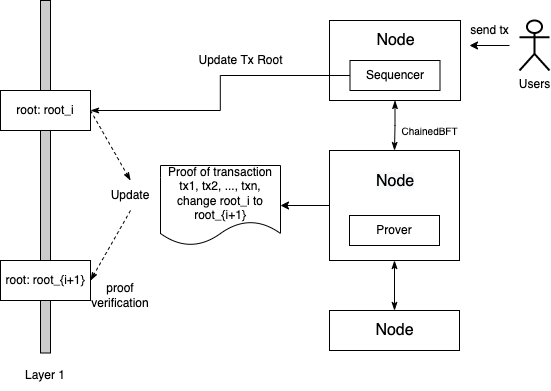
\includegraphics[width=0.6\textwidth]{arch2.drawio.png}
    \caption{\label{fig:rollup}The Rollup mechanism}
\end{figure}

~\\
\noindent\textbf{Node}. The Nodes provide the standard RPC service for users to interact ZKZRU with native Wallet, like \href{https://secret.eigen.cash}{EigenSecret}, or Metamask. The node would maintain a transaction pool, and execute the Proof-of-Proving model to reach an consensus of the order of the transactions, and submit the transaction Merkle root in L1 Rollup contract.

\begin{itemize}
    \item Sequencer: The sequencers are designed to sort the transaction by PoS consensus, and submit the transaction root into L1  after it puts down a large deposit. if that user ever submits a fraudulent batch, that deposit would be part burned and part given as a reward to the fraud prover. To realize an decentralized sequencing mechanism, we adopt ChainedBFT to reach a consensus of the transaction order in L2.
    \item Prover:  The provers are the actors that perform basic ZK Rollup functionalities. They are charged with creating blocks, making the transactions into a bundle, and performing the calculations and submitting the data to the main EVM-compatible chain for verification. The Provers retrieve a batch of transactions from L2 txpool, and generate the validity Zero-knowledge proof via EigenZkit, and submits the proof and public inputs to Rollup contract.
\end{itemize}

~\\
\noindent\textbf{Rollup contract}. The Rollup contract maintains the Rollup blockchain in L1. Once the block is produced by the Node, and submitted to the L1 Rollup contract, the \textit{updateVerifier} is a ZKRollup to verify the validity of the proof $\pi_{block}$ under the current account Merkle Tree. The main fields in the Rollup contract include:
\begin{itemize}
    \item updateNumber: uint256, block number
    \item currentRoot: uint256, merkle root of account tree
    \item updateVerifier: NIZK Verifier for validity proof verification
\end{itemize}

We define the language $L_{block}$ on algebraic composition of $L_{transfer}$ in Statement \ref{l_block}.

\begin{equation}
\begin{aligned} \label{l_block}
    L_{block} &= \wedge_{0 < i < \mbox{TX\_DEPTH}} \{  \\
        &\{((pk_s^i, pk_r^i, C_s^i, C_r^i, sk_s^i, v^i, r_1^i, r_2^i)) | \\ 
        &pk_s^i = sk_s^iG \land C_s^i = \mbox{HPKE}.Enc(pk_s^i,v^i, r_1^i) \land \\
        &C_r^i =  \mbox{HPKE}.Enc(pk_r^i,v^i, r_2^i) \land v^i \in [0, \mbox{MAX}) \land \\
        &\mbox{HPKE}.Dec(sk_s^i, \hat{C}_s^i - C_s^i) \in [0, \mbox{MAX})\}\}
\end{aligned}
\end{equation}

We translate above constraints into R1CS, transpile R1CS to Plonk Constraints, and generates the final proof $\pi_{block}$ by PlonK \cite{gabizon2019plonk}, which represents the vector of wire values as well as the different gates selectors as polynomials using interpolation. A polynomial division check ensures that the prover knows satisfying inputs and outputs for each gate, but does not ensure a correct wiring, e.g. that the output of one gate is the input to another.A permutation argument establishes the consistency of the assignment of wires to gates. The main reasons for this transpilation includes the URS setup, Pedersen Commitment/HPKE on custom gate etc.

Furthermore, the optimization for recursive proof, such as GPU-based acceleration for EC scalar multiplication and batch opening polynomial commitments, is applied to realize a very fast block validity proof verification on previous confirmed block in Rollup chain. The implementation is presented at \href{https://github.com/ieigen/EigenZKit}{EigenZKit}.


% include{zkit}
\begin{appendices}
\appendix

%\section{Borromean ring signatures on Pedersen Commitment}
%\label{appendix:borr}
%Borromean ring signatures\cite{maxwell2015borromean} 
%https://blockstream.com/bitcoin17-final41.pdf

\section{Bulletproof protocol}
\label{appendix:bp}

BulletProof doesn't depends on trust setup. BulletProof use NUMS \ref{appendex:NUMS} strategy, where a hash function is utilized to compute the generator for Pedersen Commitment. The main building block of BulletProof is Inner Product Argument(IPA). We use curve Secp256k1 in our implementation.


\begin{algorithm}
 \DontPrintSemicolon
    \caption{Compute Generator: ComputesGenerators}
    \label{alg:ComputesGenerators}
    \LinesNumbered
    
    \KwIn{The elliptic curve public generator $g \in \GG$ and an integer n.}
    \KwOut{The set of generators for Pedersen Commitment (g, h, \textbf{g}, \textbf{h})}.
    Compute h = MapToGroup('something', p) \;
    i = 0 \;
    \While {i < n} {
        $c \sample ZZ_p$ \;
        $d \sample ZZ_p$ \;
        \textbf{g}[i]=$c\cdot G$ \;
        \textbf{h}[i]=$d\cdot G$ \;
        i = i + 1\;
    }
    return (g, h, \textbf{g}, \textbf{h});
\end{algorithm}

\begin{algorithm}
 \DontPrintSemicolon
    \caption{$Setup_{IP}$}
    \label{alg:setup_ip}
    \LinesNumbered
    
    \KwIn{the set of generators(g, h, \textbf{g}, \textbf{h})}
    \KwOut{$params_{IP}$}
    
    u = MapToGroup('something', p) \;
    return $params_{IP}$ = (g, h, \textbf{g}, \textbf{h}, u)
\end{algorithm}

\begin{algorithm}
 \DontPrintSemicolon
    \caption{$Setup_{RP}$}
    \label{alg:setup_rp}
    \LinesNumbered
    
    \KwIn{the input interval [a, b), and the field modulus p}.
    \KwOut{$params_{RP}$}
    \uIf{b is not a power of 2}{
        return "b must be a power of 2"\;
    } {
        $n = log_2b$ \;
        (g, h, \textbf{g}, \textbf{h}) = ComputeGenerators(g, n) \;
        $params_{IP} = Setup_{IP}(g, h, \textbf{g}, \textbf{h})$ \;
        return $params_{RP}$ = ($params_{IP}$, n) \;
    }
\end{algorithm}

\begin{algorithm}
 \DontPrintSemicolon
    \caption{Vector Commitment: $Commit_{IP}$}
    \label{alg:vector_commitment}
    \LinesNumbered
    
    \KwIn{$params_{IP}$, \textbf{a, b}}.
    \KwOut{The commitment C}
    Compute C = $g^ah^b \in \GG$ \;
    return C.
\end{algorithm}

\begin{algorithm}
 \DontPrintSemicolon
    \caption{Prove of Inner Product: $Prove_{IP}$}
    \label{alg:prove_ip}
    \LinesNumbered
    
    \KwIn{$params_{IP}, commit_{IP}$,c, \textbf{a, b}}.
    \KwOut{$proof_{IP}$}
    x = Hash(\textbf{g, h}, P, c) $\in \GG$ \;
    Compute P' = $u^{x\cdot c}P$ \;
    Allocate arrays \textbf{l, r} $\in \GG^n$ \;
    ComputeProof(\textbf{g}, \textbf{h}, P',, $u^x$, \textbf{a, b, l, r})\;
    $proof_{IP}$ = (\textbf{g, h}, P', $u^x$, \textbf{a, b, l, r}) \; 
    return $proof_{IP}$.
\end{algorithm}

\begin{algorithm}
    \caption{Prove of Inner Product: ComputeProof}
    \label{alg:compute_proof}
    \LinesNumbered
    \KwIn{\textbf{g, h}, P, u, \textbf{a, b, l, r}}
    \KwOut{\textbf{g, h}, P, u, \textbf{a, b, l, r}}
    x = Hash(g, h, P, c $\in \ZZ_p^*$\;
    Compute P' = $u^{x\cdot c}P$ \;
    \eIf{n = 1}{
        return (\textbf{g, h}, P, u, a, b, \textbf{l, r}) \;
    } {
        n' = n/2 \;
        $C_L = <a_{[:n']}, b_{[n':]}> \in \ZZ_p$\;
        $C_R = <a_{[n':]}, b_{[:n']}> \in \ZZ_p$\;
        $L = g_{[n':]}^{a_{[:n']}} h_{[:n']}^{b_{[n':]}}u^{C_L} \in \GG$ \;
        $R = g_{[n':]}^{a_{[n':]}} h_{[n':]}^{b_{[:n']}}u^{C_R} \in \GG$ \;
        Append $L, R$ to \textbf{l, r}, respectively\;
        x = Hash($L, R$)\;
        $g' = g_{[:n']}^{x^{-1}} g_{[n':]}^{x} \in \GG^{n'}$ \;
        $h' = g_{[:n']}^{x} g_{[n':]}^{x^{-1}} \in \GG^{n'}$ \;
        $P' = L^{x^2}PR^{x^{-2}} \in \GG$ \;
        $a' = a_{[:n']}x + a_{[n':]}x^{-1} \in \ZZ_p^{n'}$ \;
        $b' = b_{[:n']}x + b_{[n':]}x^{-1} \in \ZZ_p^{n'}$ \;
        return ComputeProof(\textbf{g', h'}, P', u, \textbf{a', b', l, r})
    }
\end{algorithm}

\begin{algorithm}
 \DontPrintSemicolon
    \caption{Prove of Inner Product: $Verify_{IP}$}
    \label{alg:verify_ip}
    \LinesNumbered
    
    \KwIn{$params_{IP}, commit_{IP}, proof_{IP}$}
    \KwOut{True or false}
    
    i = 0 \;
    \While{i < logn}{
        n' = n/2 \;
        x = Hash(\textbf{l}[i], \textbf{r}[i]) \;
        $g' = g_{[:n']}^{x^{-1}} g_{[n':]}^{x} \in \GG^{n'}$ \;
        $h' = g_{[:n']}^{x} g_{[n':]}^{x^{-1}} \in \GG^{n'}$ \;
        $P' = L^{x^2}P R^{x^{-2}}\in \GG$ \;
        i = i + 1 \;
    }
    The verifier computes c = a$\cdot$ and accepts if $P = g^ah^bu^c$.
\end{algorithm}

% https://arxiv.org/pdf/1907.06381.pdf
\begin{algorithm}
 \DontPrintSemicolon
    \caption{Bulletproofs: $Prove_{RP}$}
    \label{alg:prove_rp}
    \LinesNumbered
    
    \KwIn{$params_{RP}$, v}
    \KwOut{$proof_{RP}$}
    
    $\lambda \sample \ZZ_p$ \;
    $V = g^vh^\lambda \in \GG$ \;
    $a_L \in {0, 1}^n$ s.t. $<a_L, 2^n> = v$ \;
    $a_R - a_L - 1^n \in \ZZ+p^n$ \;
    $\alpha \sample \ZZ_p$\;
    $A = h^\alpha g^{a_L}h^{a_R} \in \GG$ \;
    $s_L, s_R \sample \ZZ_p^n$\;
    $\rho \sample \ZZ_p$\;
    $S = h^\rho g^{s_L} h^{s_R} \in \GG$ \;
    $ y = Hash(A, S) \in \ZZ_p^n$ \;
    $ z = Hash(A, S, y) \in \ZZ_p^n$ \;
    $\tau_1, \tau_2 \sample \ZZ_p$ \;
    $T_1 = g^{t_1} h^{\tau_1}$ \;
    $T_2 = g^{t_2} h^{\tau_2}$ \;
    $ x = Hash(T_1, T_2) \in \ZZ_p^n$ \;
    
    \textbf{l} = $l(X) = a_L - z1^n + s_LX \in \ZZ_p^n$ \;
    \textbf{r} = $r(x) = y^n \cdot (a_R + z1^n + s_R X) + z^22^n \in \ZZ_p^n$ \;
    $\hat{t} = $ <\textbf{l, r}> $\in \ZZ_p$ \;
    $\tau_x = r_2x^2 + \tau_1 x + z^2\lambda  \in \ZZ_p$ \;
    $\mu = \alpha + \rho x \in \ZZ_p$ \;
    $commit_{IP} = Commit_{IP}(params_{IP}, l, r)$ \;
    $proof_{IP} = Prove_{IP}(params_{IP}, commit_{IP}, \hat{t}, l, r)$ \;
    return $proof_{RP} = Prove_{RP}(\tau_x, \mu, \hat{t}, V, A, S, T_1, T_2, commit_{IP}, proof_{IP})$ \;
\end{algorithm}

\begin{algorithm}
 \DontPrintSemicolon
    \caption{Bulletproofs: $Verify_{RP}$}
    \label{alg:verify_rp}
    \LinesNumbered

    \KwIn{$params_{RP}, proof_{rp}$}
    \KwOut{True or false}
    
    $ y = Hash(A, S) \in \ZZ_p^n$ \;
    $ z = Hash(A, S, y) \in \ZZ_p^n$ \;
    $ x = Hash(T_1, T_2) \in \ZZ_p^n$ \;
    
    $h_i = h_i^{y^{-i + 1}} \in \GG, \forall i \in [1, n]$\;
    $P_l = p \cdot h^\mu $\;
    $P_r = A\cdot S^x\cdot g^{-z} \cdot (h')^{z\cdot y^2 + z^2 \cdot 2^n} \in \GG$\;
    $output_1 = (P_l \overset{?}{=}P_r)$ \;
    $output_2 = (g^{\hat{t}} h^{r_x} \overset{?}{=} V^{z^2}\cdot g^{\sigma(y, z)\cdot T_1^x \cdot T_2^{x^2}})$ \;
    $output_3 = Verfify_{IP}(proof_{IP})$ \;
    return $output_1 \land output_2 \land output_3$ 
\end{algorithm}

\section{Boneh-Boyen Signatures without pairings}
\label{appendex: bbs-no-pairing}
Boneh-Boyen Signatures scheme \cite{jao2009boneh} used by the designated authority
(which could be the verifier) to sign each element of the set $\Phi$ is the one proposed by Boneh and Boyen.
Based on this scheme, which is secure under the q-SDH assumption, it is possible to prove knowledge of a
signature on a message, without revealing the signature nor the message.

For a given secret x, and two random generatos $g_1, g_2$ of $G_1$, the signature of a message $m \in \ZZ_p$ is obtained by computing $\sigma = g_1^{1/(x+m)}$. Given a bilinear pairing e, a signature $\sigma$ of m is valid if $e(\sigma, yg_2^m) = e(g_1, g_2)$ holds, where $y = g_2^x$.

\cite{arfaoui2015practical} proposed BB signature without pairing under the DDH assumption. Let G be a cyclic group with prime order p where the
Decisional Diffie-Hellman (DDH) problem is assumed to be hard and $g_1, g_2$ two random generators of $\GG$. The signer’s private key is $x \in \ZZ_p$ and it's public key is $y = g^x$, so the signature would be $\sigma = g_1^{1/(x+m)}$, which implies that $A^x = g_1 A^{-m}$. So the signer can prove the signature is valid by generating a ZKPK $\pi$:
\begin{equation}
    SOK(x: X = g_2^x \land A^x = g_1A^{-m})
\end{equation}
which means the discrete logarithm of ($g_1 A^{-m}$) in the base A is equal to the discrete logarithm of $x$ in the base $g_2$.

\section{Set Membership Proof on BB Signature without pairing}

\begin{myDef}
\label{d5}
\textbf{Borreomean ring signature\cite{maxwell2015borromean}} let $\mathcal{V}$ be some set of verification keys, and f be a function which maps finite subsets of $\mathcal{V}$ to ${0, 1}$, we call f an admissibility function, then an admissible set V of verification keys is one for which f($\mathcal{V}$) = 1. 

A Borromean ring signature $\sigma$ is a signature on a message m with a set V of verification keys and admissibility function f which satisfy the following:
\begin{enumerate}
    \item $\sigma$ can be produced only by parties who together know all the secret keys to an admissible set $\mathcal{V}$ of verification keys.
    \item Given only $\sigma$ , $\mathcal{V}$ , and $m$, it is statistically indistinguishable which admissible set V was used.
\end{enumerate}
\end{myDef}

Proving knowledge of a valid BB Signature $A_k = g^{1/{y+k}}$ on a value $k$ commited in $Com = g_1^k h^v$, without using parings on the prover's side can be done in Algorithm \ref{alg:prove_sm} and Algorithm \ref{alg:verify_sm}. 

\begin{algorithm}
 \caption{Set Membership Proof: $Prove_{SM}$}
    \label{alg:prove_sm}
    \LinesNumbered
    
    \KwIn{challenge $ch$, public input=(set $\Phi$), private input = ($k, A_k = g^{1/{y+k}}$)}
    \KwOut{$proof_{SM}$}
    
    $v \sample \ZZ_p^*$\;
    $Com = g_1^k h^v$ \;
    $A_k = g^{1/(y+k)}$ \;
    $l \sample \ZZ_p^*$ \;
    $B = A_k^l, B_1 = B^{-1}, D = B_1^kg^l$ \;
    $k_1, l_1, r_1 \sample \ZZ_p^*$ \;
    $Com_1 = g_1^{k_1}h^{r_1}, D_1 = B_1^{k_1} g^{l_1}$ \;
    
    $C = H(Com, B, D, Com_1, D_1, ch)$ \;
    $s_1 = k_1 + c \times k \mod p$ \;
    $s_2 = r_1 + c \times r \mod p$ \;
    $s_3 = l_1 + c \times l \mod p$ \;
    
    $proof_{SM} = (Com, B, D, s_1, s_2, s_3)$
\end{algorithm}

\begin{algorithm}
 \caption{Set Membership Proof: $Verify_{SM}$}
    \label{alg:verify_sm}
    \LinesNumbered
    
    \KwIn{challenge $ch$, $proof_{SM}$}
    \KwOut{True or false}
    
    $\hat{C} = g_1^{s_1}h^{s_2}, \hat{D} = B_1^{s_1}g^{s_3}D^{-c}$ \;
    $output_1 = B \neq 1_{G_1}$ \;
    $output_2 = H(Com, B, D, \hat{C}, \hat{D}, ch)$ \;
    
    return $output_1 \land output_2$
\end{algorithm}

\section{Nothing Up My Sleeve}
\label{appendex:NUMS}
This method enables the generation of verifiable random values. NUMS allows a prover to pick values in a way that demonstrates the values were not selected for a "nefarious purpose" - for example, to create a "backdoor" to the algorithm \cite{black2014elliptic}. The algorithm on curve Secp256k1 is described in Algorithm \ref{alg:nums}.

\begin{algorithm}
 \caption{Nothing Up My Sleeve: MapToGroup}
    \label{alg:nums}
    \LinesNumbered
    
    \KwIn{The input string m, and the filed prime modules p}
    \KwOut{AN elliptic curve point if successful or some error}
    i = 0 \;
    \While {i < 256} {
        x = Hash(m, i) \;
        rhs = $x^3 + 7$ \;
        \uIf {rhs is a sqaure (mod p) } {
            $y = \sqrt{rhs}$ mod p \;
            \uIf{(x, y) is not the point at infinity}{
                return (x, y) \;
            }
        }
        i = i + 1\;
    }
    return "Can not map to group"\;
\end{algorithm}
\end{appendices}


\bibliographystyle{alpha}
\bibliography{ref}

\end{document}